\section{Задание 3. Приложения и пакеты в Ubuntu}

Работа с пакетами способы установки приложений \ref{fig:installChrome} :

\begin{figure}[!h]
    \centering
    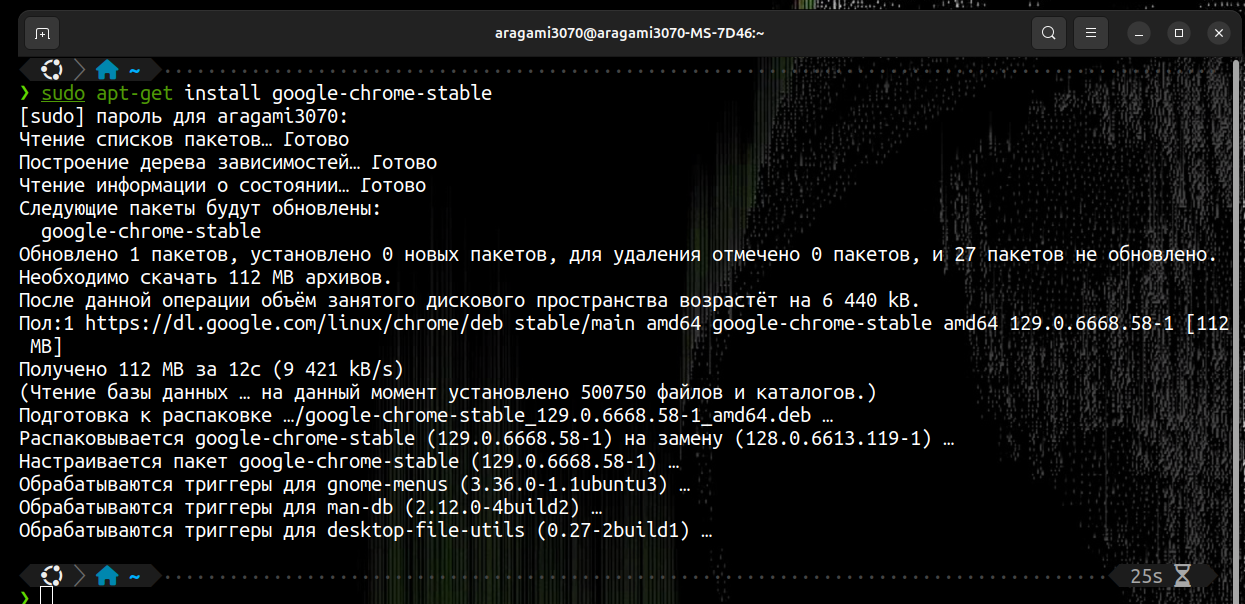
\includegraphics[width = 0.8\textwidth]{images/installChrome.png}
    
    \caption{Установка chrome}
    
    \label{fig:installChrome}
\end{figure}

Установка через Ubuntu Software Center \ref{fig:installDiscord} :

\begin{figure}[!h]
    \centering
    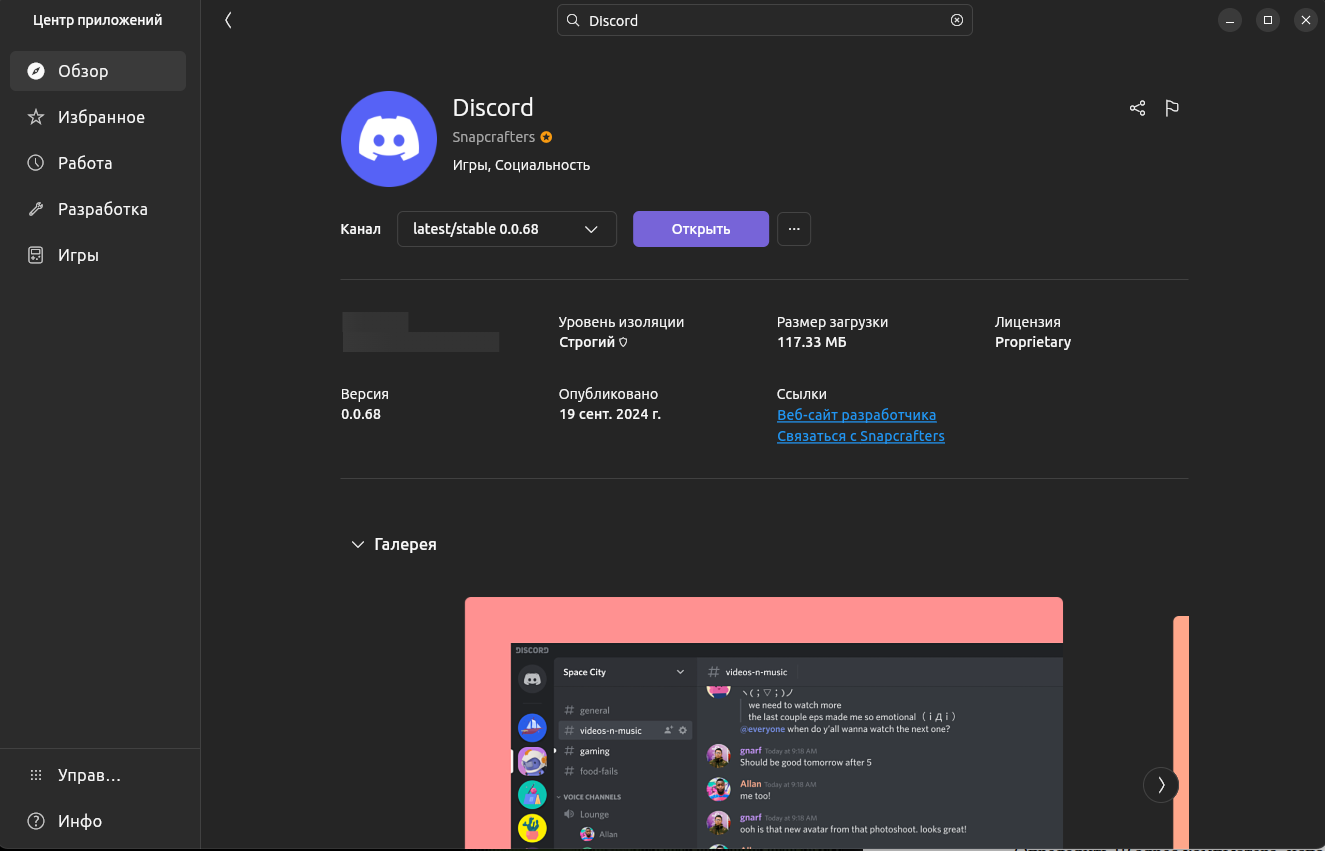
\includegraphics[width = 0.7\textwidth]{images/installDiscord.png}
    
    \caption{Установка через Ubuntu}
    
    \label{fig:installDiscord}
\end{figure}

\newpage

Установка/удаление популярных приложений \ref{fig:installDelVScode} \ref{fig:delChrome}:

\begin{figure}[!h]
    \centering
    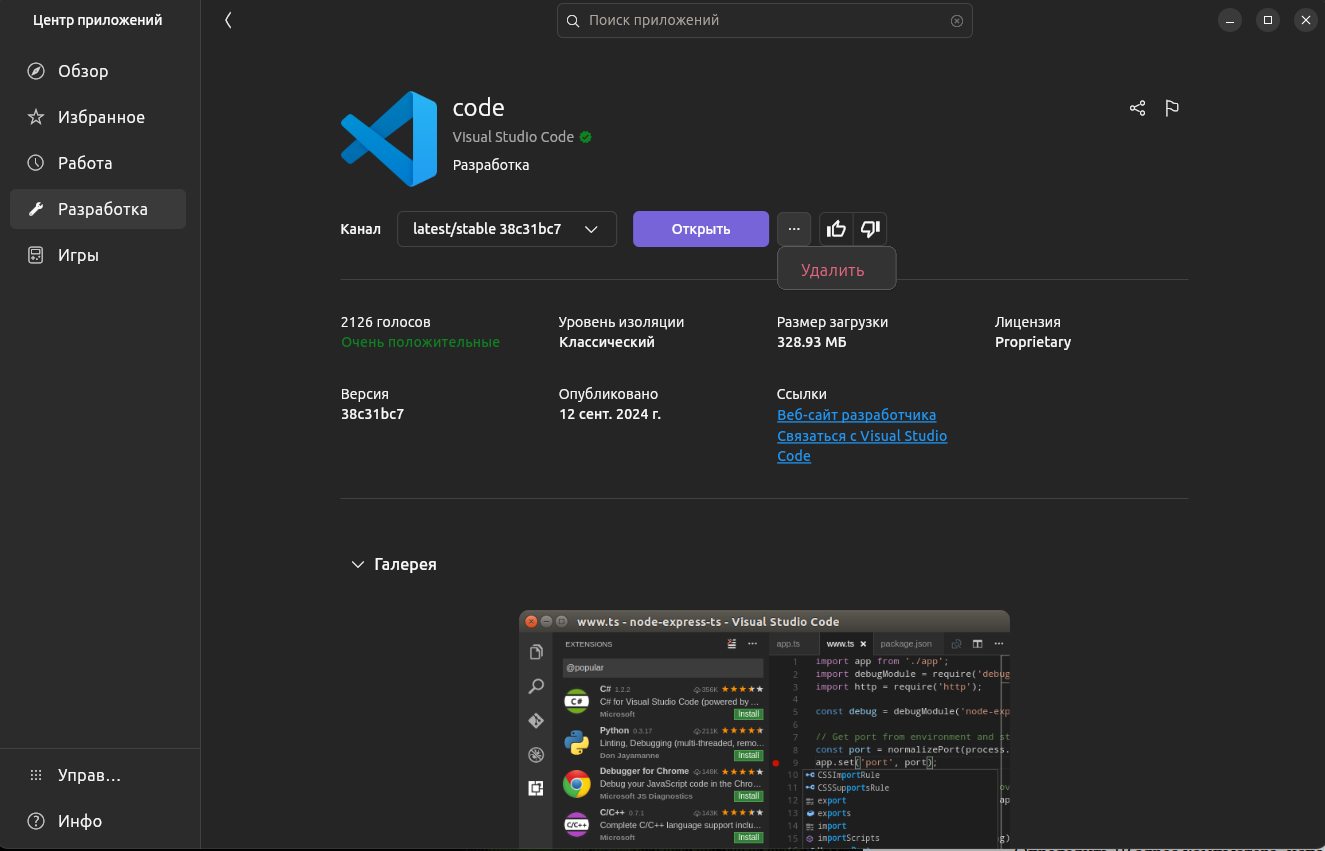
\includegraphics[width = 0.8\textwidth]{images/installDelVScode.png}
    
    \caption{установка/удаление через Ubuntu Software Center}
    
    \label{fig:installDelVScode}
\end{figure}

\begin{figure}[!h]
    \centering
    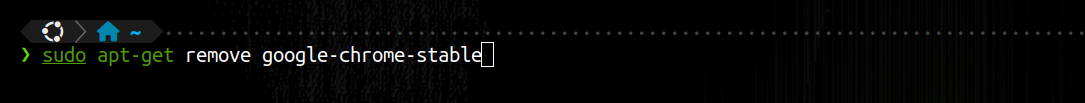
\includegraphics[width = 0.8\textwidth]{images/delChrome.png}
    
    \caption{удаление через терминал}
    
    \label{fig:delChrome}
\end{figure}
